\documentclass[journal ]{new-aiaa}
\usepackage[utf8]{inputenc}
\usepackage{textcomp}
\usepackage{subcaption}
\usepackage{float}

\usepackage{graphicx}
\usepackage{amsmath}
\usepackage[version=4]{mhchem}
\usepackage{siunitx}
\usepackage{longtable,tabularx}
\setlength\LTleft{0pt} 

\title{Optimization of Multiple Rotors}

\author{J. Spencerr \footnote{Undergraduate Researcher, Brigham Young University FLOW Lab.}}
\affil{Brigham Young University, Provo, Utah, 84601} % Other authors are listed in the same way

\begin{document}

\maketitle

\begin{abstract}
This report describes a project completed as part of my research with the Brigham Young University FLOW Lab. this project drew on skills gained throughout the semester to design and execute a code in the Julia programming language to find the optimal blade count, blade thickness magnification, and twist angle for a propellor to achieve its maximum efficiency, $\eta$, at a known advance ratio, $J$. This investigation found that thinner rotors are more efficient, especially at negative angles of attack. The implications of these results and possible areas of future research are then discussed.

\end{abstract}


\section*{Nomenclature}

\noindent(Nomenclature entries are identified with their default units.)

{\renewcommand\arraystretch{1.0}
\noindent\begin{longtable*}{@{}l @{\quad=\quad} l@{}}

$J$ & Advance Ratio, \emph{dimensionless} \\
$\alpha$ & Angle of Attack, $rad$ \\
$\phi$ & Angle of Rotation, $rad$ \\
$\Omega$ & Angular Speed, $rev./s$ \\
$W$ & Apparent Speed, $m/s$ \\
$a$ & Axial Induction Factor \emph{dimensionless} \\
$M_{b}$ & Bending Moment, $N \times m$ \\
$r$ & Blade Tip Radius, $m$ \\
$c$ & Chord length, $m$ \\
$D$ & Diameter, $m$ \\
$c_{d}$ & Drag Coefficient, \emph{dimensionless} \\
$D$ & Drag Force, $N$ \\
$\nu$ & Dynamic Viscosity, $\frac{N s}{m^{2}}$ \\
$\eta$ & Efficiency, \emph{unitless} \\
$\rho$ & Fluid Density, $kg/m^{3}$ \\
$v_{a}$, $U_{\infty}$ & Freestream Velocity, $m/s$ \\
$\mu$ & Kinematic Viscosity, $m^{2}/s$ \\
$c_{l}$ & Lift Coefficient, \emph{dimensionless} \\
$L$ & Lift Force, $N$ \\
$M$ & Mach Number, \emph{dimensionless} \\
$M_{p}$ & Pitching Moment, $N \times m$ \\
$c_{m}$ & Pitching Moment Coefficient, \emph{dimensionless} \\
$P$ & Power, $W$ \\
$C_{P}$ & Power Coefficient, \emph{dimensionless} \\
$N$ & Propellor Count, \emph{integer} \\
$\omega$ & Radial Velocity, $\frac{rad.}{s}$ \\
$RPM$ & Revolutions Per Minute, $\frac{\emph{rev.}}{\emph{min.}}$ \\
$Re$ & Reynolds Number, \emph{dimensionless} \\
$n$ & Rotational Frequency, $\frac{rev.}{s}$ \\
$\sigma$ & Rotor Solidity \emph{dimensionless} \\
$n$ & Safety Factor, \emph{dimensionless} \\
$s$ & Spacing, $m$ \\
$A$ & Surface Area, $m${2} \\
$\beta$ & Stationary Angle of Rotation, $rad.$ \\
$a'$ & Tangential Induction Factor \emph{dimensionless} \\
$T$ & Thrust, $N$ \\
$C_{T}$ & Thrust Coefficient, \emph{dimensionless} \\
$\lambda$ & Tip Speed Ratio, \emph{dimensionless} \\
$Q$ & Torque, $N \times m$ \\
$C_{Q}$ & Torque Coefficient, \emph{unitless} \\
$v_{i}$ & Uniform Induced Velocity, $m/s$ \\
$u$ & Velocity, $m/s$ \\

\end{longtable*}}


\section{Introduction}

\lettrine{P}{ropellors} come in a variety of different shapes and sizes. This paper describes how one propellor, which started as an APC 10x7 rotor and a NACA 4412 airfoil, was optimized to perform better at a certain advance ratio. The code used for this report could also be applied to different rotors in the future.

This report shows how computer simulations can be used to simulate the performance of propellors without needing to actually create them. It finds that changing the twist angle and the thickness of a propellor shifts the curves for its efficiency, thrust coefficient, and torque coefficient, and that propellors with different blade counts also have different curves for these three non-dimensional numbers. All code used for each section of this report can also be accessed through a GitHub repository \footnote{This repository can be accessed at \url{https://github.com/JoeSpencer1/497R-Projects}}.


\section{Procedure}

This project was performed using julia programming language. \footnote{julia can be found at \url{https://julialang.org}.} jula is available for free and is useful for a variety of reasons. It can store data as vectors and matrices, and perform rapid calculations with these objects. It compiles functions in advance, so they can be run more quickly than other languages like python. Header files needed for this project, including Xfoil \footnote{Xfoil.jl is available at \url{https://github.com/byuflowlab/Xfoil.jl}}, CCBlade \footnote{CCBlade.jl is available at \url{https://github.com/byuflowlab/CCBlade.jl}}, SNOW \footnote{SNOW.jl is available at \url{https://github.com/byuflowlab/SNOWl.jl}}, and FLOWMath \footnote{FLOWMath.jl is available at \url{https://github.com/byuflowlab/FLOWMath.jl}}, are all designed for julia. These files provided useful functionality that simplified the design process.

In the rotor design process, an airfoil was first created using Xfoil.jl. This rotor was then attached to a rotor and evaluated using CCBlade.jl. Data about the rotor, including its moments in the normal and tangential directions and its torque, is recorded. This data is then multiplied by a factor, in this case $n=1.1$, to determine the maximum allowable loads before the rotor would break or a different material would be required. After constraints are determined, rotor variable types called \emph{rotortest} are created with variable thickness magnification and rotation angle and the program uses Optim.jl to find the rotor with the optimal twist angle and thickness magnification for the objective function.

The objective function used in this optimization is listed in equation 1. 

\begin{equation}
	\begin{aligned}
	\label{equation:1}
	f(x_{1}, x_{2}, x_{3}...) = \eta \\
	\end{aligned}
\end{equation}.

Constraints were placed on the solution to ensure that the optimizer found a reasonable solution. In addition to restrictions on the moment and torque, the cord thickness was kept within a factor of two of the original and the twist angle magnitde was kept below $90^{\circ}$

\begin{center}
\begin{tabular}{l  r}
	 \multicolumn{2}{c}{Table 1: Optimization objective, parameters, and constraints}  \\
  	Maximize: & $\eta$ \\ \hline
  	By varying: & scale of the chord, $c$ \\ 
  	 & twist angle, $\phi$ \\  \hline
  	Subject to & total torque less than 110\% of original \\ 
	 & normal moment less than 110\% of original \\ 
	 & tangential moment less than 110\% of original \\ 
	 & $-90^{\circ} <$ twist angle $< 90^{\circ}$ \\
	 & $50\% <$ chord magnification $< 200\% $
\end{tabular} \newline
\end{center}



\section{Results}

As stated previously, an APC 10x7 rotor with what started as a NACA 4412 airfoil was optimized. While the APC rotor number stayed the same, the NACA airfoil number was changed. The maximum chord found in first digit and the maximum thickness from two digits at the end are multiplied by whatever the magnification of the chord is. So, a NACA 4412 airfoil becomes a NACA 2206 airfoil at 50\% magnification and a NACA 8424 at 200\%.

The propellor was checked at blade counts of 2, 3, and 4. These results are described and compared in plot 1. This report found that for all three blade counts, the optimal propellor was as thin as possible, with negative angles of attack. The finding about thinner rotor blades being more efficient was in line with \textbf{THE PAPER} \footnote{Experimental study of blade thickness effects on the overall and local performances of a Controlled Vortex Designed axial-flow fan, \url{https://doi.org/10.1016/j.expthermflusci.2011.01.002}}, but such a high negative rotation angle was surprising.

\subsection{Results Table}

Table 2 shows the optimal twist angles and chord magnifications for each different rotor blade count. The reader can observe that the optimal thickness for each propellor blade was the very thinnest possible. The thickness had to between 50\% and 200\% of the original. The optimal angle of rotation was slightly less than $-10^(\circ)$ for each rotor, gradually decreasing in magnitude as the blade count increased.

\begin{center}
\begin{tabular}{| c | c | c |}
	 \multicolumn{3}{c}{Table 2: Optimized Chord Magnification and Rotation Angles for Different Blade Counts}  \\ \hline
  	 \textbf{Blade Count} & \textbf{Chord Thickness Multiplication} & \textbf{Twist Angle} \\ \hline
  	 3 (Default) & 1.0 & $0^{\circ}$ \\ \hline
  	 2 & 0.50 & $-9.54^{\circ}$ \\ \hline
  	 3 & 0.50 & $-9.47^{\circ}$ \\ \hline
  	 4 & 0.50 & $-9.39^{\circ}$ \\ \hline
\end{tabular}
\end{center}

\subsection{Results Plot}

Four plots, displayed below, were output by the rotor analysis. Figure 1 shows that while the optimized design increased the efficiency of even the rotor with a higher blade count above the rotor pre-optimization, it 

\begin{figure}[H]
\centering
 	\subfloat[Efficiency]{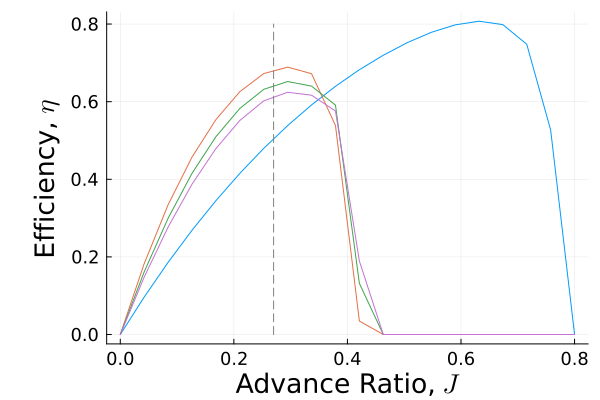
\includegraphics[width = .40\textwidth]{Plots/Figure_1.png}}
	\subfloat[Thrust Coefficient]{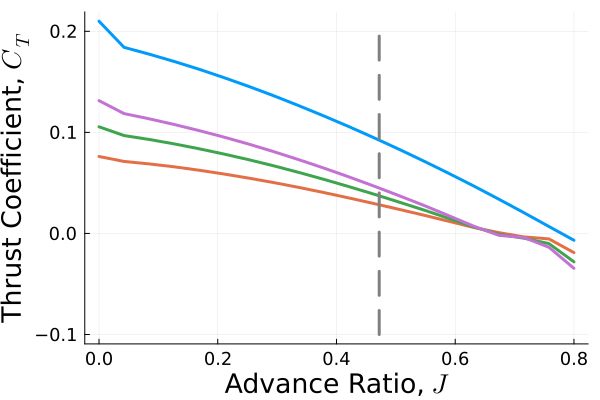
\includegraphics[width = .40\textwidth]{Plots/Figure_2.png}}

	\subfloat[Torque Coefficient]{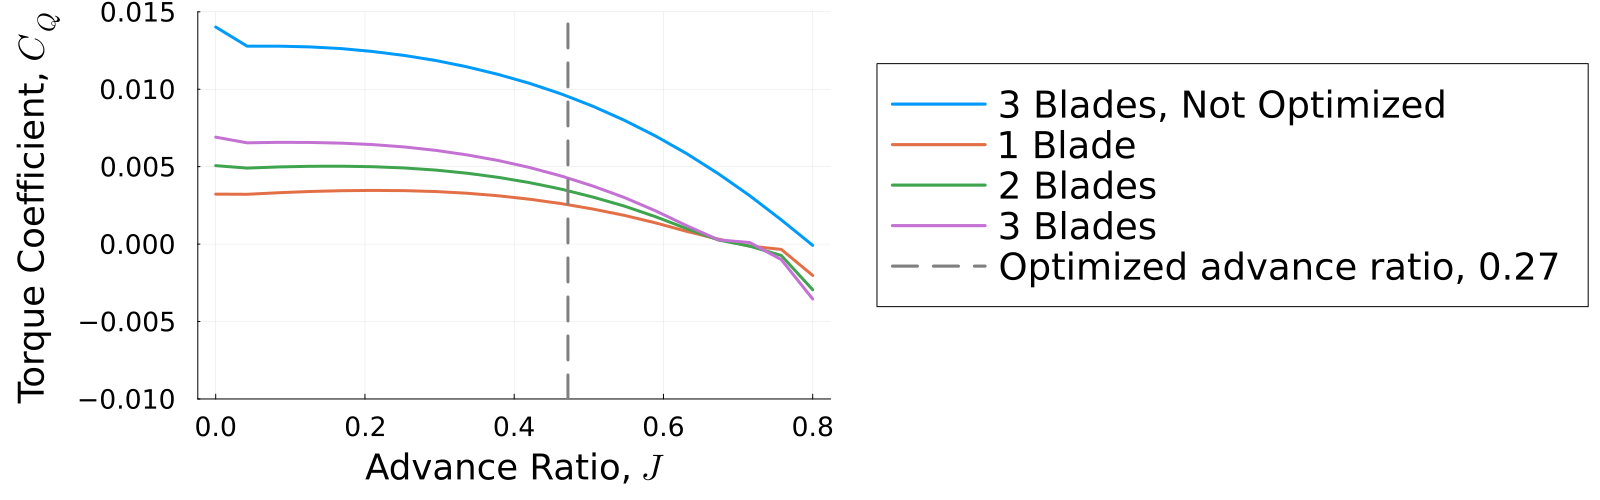
\includegraphics[width = .80\textwidth]{Plots/Figure_3.png}}\hspace{1em}
	\caption{Efficiency, Thrust Coefficients, and Torque Coefficients Compared at Different Advance Ratios}
	\captionsetup{aboveskip=0pt,font=it}
	\caption*{These plots visually represent how optimized rotors are different from the original rotor.}
	\label{fig:1}
\end{figure}



\subsection{Publication Charges for Open Access}

Publication charges are voluntary, and nonpayment has no influence on the review process of the time from acceptance to publication. The article publication charge for immediate Open Access is available in ScholarOne and on the AIAA website; the fee is the same regardless of article type.


\section{Instructions}

If you are using the AIAA Journals \LaTeX{} Template file to prepare your manuscript, you can simply type your own text over sections of this document, or cut and paste from another document and use the available markup styles. If you choose to cut and paste, select the text from your original document and choose Edit>Copy. (Do not select your title and author information, since the document spacing may be affected. It is a simple task to reenter your title and author information in the template.) Open the Journals Template. Place your cursor in the text area of the template and select Edit>Paste. Please note that special formatting (e.g., subscripts, superscripts, italics) may be lost when you copy your text into the template.

To apply the AIAA Journals formatting, use the standard \LaTeX{} commands for sections and subsection, etc; all the styles you will need to format your document are available as standard \LaTeX{} commands. The style will automatically adjust your fonts and line spacing. Repeat this process to apply formatting to all elements of your paper. \emph{Do not change the font sizes, line spacing, or margins. Do not manually hyphenate your document.} Use italics for emphasis; do not underline. 

Use the Print option under the File tab to view Page Layout and see the most accurate representation of how your final paper will appear. Once formatting is complete, be sure to double space all sections of your manuscript.


\subsection{Document Text}
The default font for the Template is Times New Roman, 10-point size. The first line of every paragraph should be indented, and all lines should be double-spaced. Default margins are 1 in. on all sides. In the electronic version of this template, all margins and other formatting are preset. There should be no additional (blank) lines between paragraphs.

\emph{NOTE:} If you are using the Template to format your manuscript, the required spacing and formatting will be applied automatically.


\subsection{Headings}
Format the title of your paper in bold, 18-point type, with capital and lower-case letters, and center it at the top of the page. The names of the authors, business or academic affiliation, city, and state/province follow on separate lines below the title. The names of authors with the same affiliation can be listed on the same line above their collective affiliation information. Author names are centered, and affiliations are centered and in italic type. The affiliation line for each author includes that author’s city, state, and zip/postal code (or city, province, zip/postal code and country, as appropriate). The first footnote (bottom of first page) contains the job title and department name, and AIAA member grade for each author. Author email addresses may be included also.

Major headings in the template (``sections'' in the \LaTeX{} template commands) are bold 11-point font and centered. Please omit section numbers before all headings unless you refer frequently to different sections. Use Roman numerals for major headings if they must be numbered.

Subheadings (``subsections'' in the \LaTeX{} template commands) are bold, flush left, and either unnumbered or identified with capital letters if necessary for cross-referencing sections within the paper. There must be at least 2 of all subheadings and sub-subheadings. If there is only a single subheading or sub-subheading, please italicize the title of the subheadings, followed by a period, and run it into the text paragraph. 

Sub-subheadings (``subsubsections'' in the \LaTeX{} template commands) are italic, flush left, and either unnumbered or numbered with Arabic numerals (1, 2, 3, etc.) if necessary for cross-referencing sections within the paper.


\subsection{Abstract}
An abstract appears at the beginning of Full-Length Papers, Regular Articles, and Express Articles. (Survey and Design Forum Papers, History of Key Technologies Papers, invited lectures, and Technical/Engineering Notes do not include abstracts.) The abstract is one paragraph (not an introduction) and complete in itself (no reference numbers). It should indicate subjects dealt with in the paper and state the objectives of the investigation. Newly observed facts and conclusions of the experiment or argument discussed in the paper must be stated in summary form; readers should not have to read the paper to understand the abstract. Format the abstract bold, indented 3 picas (1/2 in.) on each side, and separated from the rest of the document by two blank lines.


\subsection{Nomenclature}
Papers with many symbols may benefit from a nomenclature list that defines all symbols with units, inserted between the abstract and the introduction. If one is used, it must contain all the symbology used in the manuscript, and the definitions should not be repeated in the text. In all cases, identify the symbols used if they are not widely recognized in the profession. Define acronyms in the text, not in the nomenclature. 

\subsection{Biographies}
Survey Papers and some Full-Length Papers include author biographies. These biographies are one paragraph each and should use the abstract formatting style.

\subsection{Footnotes and References}
Footnotes, where they appear, should be placed above the 1'' margin at the bottom of the page. Numbered footnotes are acceptable, but superscript symbols are the preferred AIAA style, in the sequence, *, $\dag$, $\ddag$, \S, \P, **, $\dag\dag$, $\ddag\ddag$, \S\S, etc.

List and number all references at the end of the paper. Corresponding bracketed numbers are used to cite references in the text \cite{vatistas1986reverse}, including citations that are an integral part of the sentence (e.g., ``It is shown in \cite{dornheim1996planetary} that\ldots '') or follow a mathematical expression: ``$A^{2} + B = C$ (Ref.~\cite{terster1997nasa}).'' For multiple citations, separate reference numbers with commas \cite{peyret2012computational,oates1997aerothermodynamics}, or use a dash to show a range \cite{volpe1994techniques,thompsonspacecraft,chi1993fluid,brandis2016nonequi}. Reference citations in the text should be in numerical order. 

In the reference list, give all authors' names; do not use ``et al.''. Papers that have not been published should be cited as ``unpublished''; papers that have been submitted or accepted for publication should be cited as ``submitted for publication.'' Private communications and personal website should appear as footnotes rather than in the reference list.

References should be cited according to the standard publication reference style (for examples, see the ``References'' section of this template). Never edit titles in references to conform to AIAA style of spellings, abbreviations, etc. Names and locations of publishers should be listed; month and year should be included for reports and papers. For papers published in translation journals, please give the English citation first, followed by the original foreign language citation.

\subsection{Figures and Tables}
Insert tables and figures within your document; they may be either scattered throughout the text or grouped all together at the end of the file. Do not insert your figures in text boxes. Figures should have no background, borders, or outlines. In the \LaTeX{} template, use the ``caption'' command to type caption text. Captions are bold with a single tab (no hyphen or other character) between the figure number and figure description. See the Table 1 example for table style and column alignment. If you wish to center tables that do not fill the width of the page, simply highlight and “grab” the entire table to move it into proper position.


\begin{table}[hbt!]
\caption{\label{tab:table1} Transitions selected for thermometry}
\centering
\begin{tabular}{lcccccc}
\hline
& Transition& & \multicolumn{2}{c}{}\\\cline{2-2}
Line& $\nu''$& & $J'' $& Frequency, cm$^{-1}$& $FJ$, cm$^{-1}$& $G\nu $, cm$^{-1}$\\\hline
a& 0& P$_{12}$& 2.5& 44069.416& 73.58& 948.66\\
b& 1& R$_{2}$& 2.5& 42229.348& 73.41& 2824.76\\
c& 2& R$_{21}$& 805& 40562.179& 71.37& 4672.68\\
d& 0& R$_{2}$& 23.5& 42516.527& 1045.85& 948.76\\
\hline
\end{tabular}
\end{table}


\begin{figure}[hbt!]
\centering
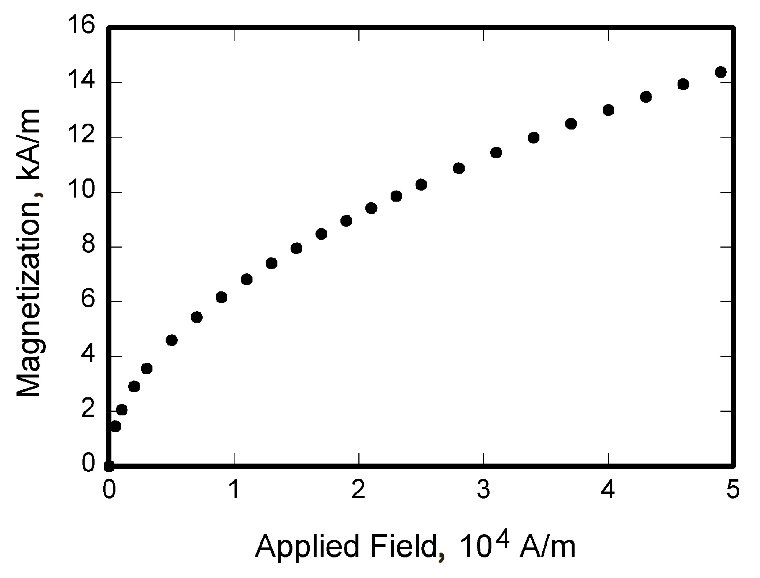
\includegraphics[width=.5\textwidth]{graph}
\caption{Magnetization as a function of applied fields.}
\end{figure}

Line drawings must be clear and sharp. Make sure that all lines and graph points are dark and distinct and that lettering is legible. Keep the lettering size and style uniform both within each figure and throughout all of your illustrations, no smaller than 8- to 10-point type for artwork that is sized to fit the column width (3\,\textonequarter{} in.)~or the full-page width (7\,in.). Place figure captions below each figure, and limit main caption length to 20--25 words. If your figure has multiple parts, include the labels “a),” “b),” etc., below and to the left of each part, above the figure caption. Please verify that the figures and tables you mention in the text actually exist. When citing a figure in the text, use the abbreviation “Fig.” except at the beginning of a sentence. Do not abbreviate “Table.” Number each different type of illustration (i.e., figures and tables) sequentially with relation to other illustrations of the same type.

Figures that are slightly wider than the column width will be reduced in size to fit, so ensure that labels will remain legible (no smaller than 8 to 10 points) after reduction to column width. 

All tables are numbered consecutively and must be cited in the text; give each table a definitive title. Be sure that you have a minimum of two columns (with headings) and two rows to constitute a proper table; otherwise reformat as a displayed list or incorporate the data into the text. Plan tables to fit the column width (3 ¼ in.) or the journal page width (7 in.). Position a double rule at the top and bottom of each table and single rule under the column headings; do not use shading, border lines, or vertical rules between table columns. Position each table in the text close to where it is cited


\subsection{Equations}
Equations are numbered consecutively, with equation numbers in parentheses flush right, as in Eq.~\eqref{sample:equation}. Insert a blank line on either side of the equation. To insert an equation into the \LaTeX{} document, use the \verb|\begin{equation}...\end{equation}| command environment.

A sample equation is included here, formatted using the preceding instructions:

\begin{equation}
\label{sample:equation}
\int^{r_2}_0 F(r,\varphi){\rm d}r\,{\rm d}\varphi = [\sigma r_2/(2\mu_0)]\int^{\infty}_0\exp(-\lambda|z_j-z_i|)\lambda^{-1}J_1 (\lambda r_2)J_0 (\lambda r_i\,\lambda {\rm d}\lambda)
\end{equation}

Be sure that symbols in your equation are defined in the Nomenclature or immediately following the equation. Also define abbreviations and acronyms the first time they are used in the main text. (Very common abbreviations such as AIAA and NASA, do not have to be defined.)

\subsection{General Grammar and Preferred Usage}
Use only one space after periods or colons. Hyphenate complex modifiers: ``zero-field-cooled magnetization.'' Insert a zero before decimal points: ``0.25,'' not ``.25.'' Use ``\si{\centi\meter\squared}'' not ``cc.'' 

A parenthetical statement at the end of a sentence is punctuated outside of the closing parenthesis (like this). (A parenthetical sentence is punctuated within parenthesis.) Use American, not English, spellings (e.g., “color,” not “colour”). The serial comma is preferred: “A, B, and C” instead of “A, B and C.”

Be aware of the different meanings of the homophones “affect” (usually a verb) and “effect” (usually a noun), “complement” and “compliment,” “discreet” and “discrete,” “principal” (e.g., “principal investigator”) and “principle” (e.g., “principle of measurement”). Do not confuse “imply” and “infer.”

\section{Conclusion}
Although a conclusion may review the main points of the paper, it must not replicate the abstract. A conclusion might elaborate on the importance of the work or suggest applications and extensions. Do not cite references in the conclusion. Note that the conclusion section is the last section of the paper to be numbered. The appendix (if present), funding information, other acknowledgments, and references are listed without numbers.

\section*{Appendix}

An Appendix, if needed, appears \textbf{before} research funding information and other acknowledgments.

\section*{Funding Sources}

Sponsorship information and acknowledgments of financial support should be included here. \textbf{Authors are responsible for accurately reporting funding data relevant to their research.} Please confirm that you have correctly entered \textbf{all sources} of funding and grant/award numbers \textbf{for all authors} in this section of your article. You will also be asked to select the appropriate funding organization from a drop-down menu in ScholarOne when you submit your manuscript. Be careful to choose the correct funder name, as organization names can be similar, and also be mindful to select sub-organizations within the registry hierarchy that are the actual funding sources, as appropriate, rather than choosing the name of the parent organization. Information provided in your manuscript must match the funding data entered in ScholarOne.

\section*{Acknowledgments}
An Acknowledgments section, if used, \textbf{immediately precedes} the References. Individuals other than the authors who contributed to the underlying research may be acknowledged in this section. The use of special facilities and other resources also may be acknowledged. 

\bibliography{Final_Report}

\end{document}
